\begin{figure}[h][p]
    \centering
    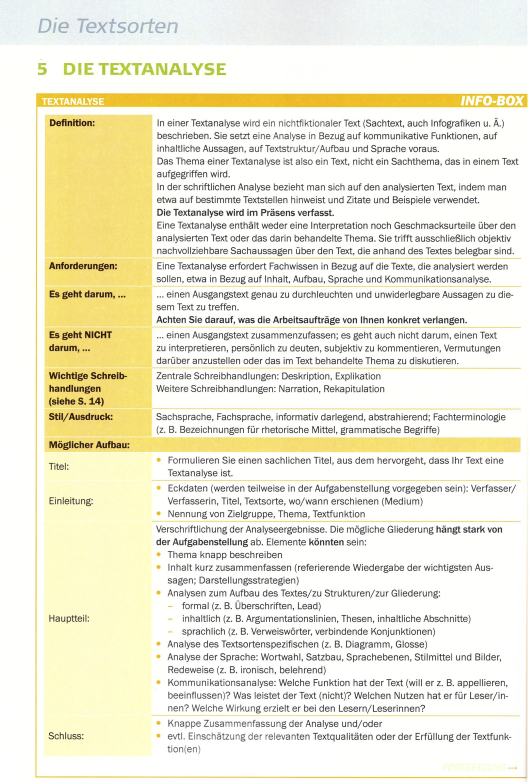
\includegraphics[scale=0.8]{pics/Screenshot from 2023-02-06 12-30-44.png}
    \caption{Textanalyse: Definition + Aufbau}
    \label{fig:impl:Textanalyse1}
\end{figure}

\begin{figure}[h][p]
    \centering
    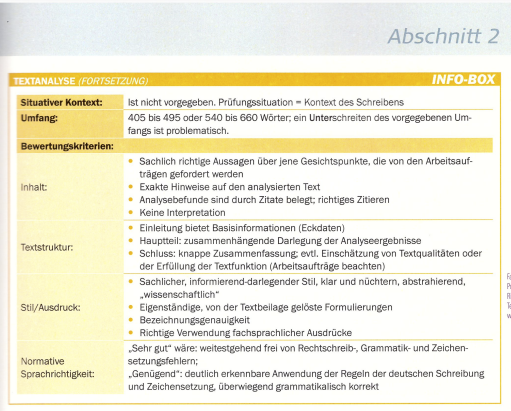
\includegraphics[scale=0.8]{pics/Screenshot from 2023-02-06 12-30-55.png}
    \caption{Textanalyse: Verfassen}
    \label{fig:impl:Textanalyse2}
\end{figure}
\begin{figure}[h][p]
    \centering
    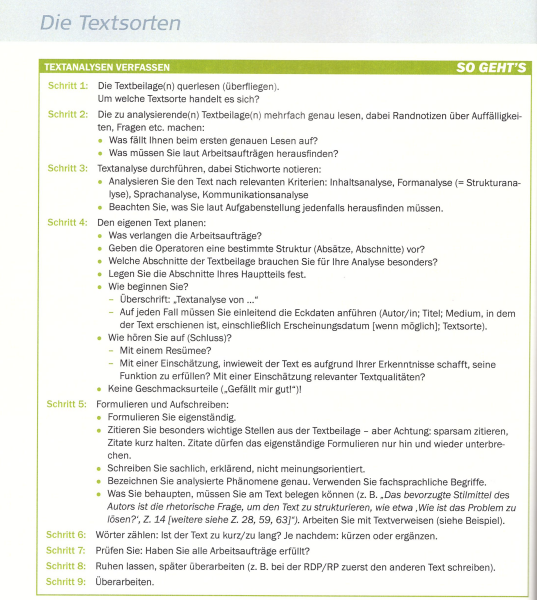
\includegraphics[scale=0.8]{pics/Screenshot from 2023-02-06 12-31-09.png}
    \caption{Textanalyse: Fortsetzung}
    \label{fig:impl:Textanalyse3}
\end{figure}

\section{Mustertext}
\subsubsection{Textanalyse: „Der Unsinn von der „Work-Life-Balance“}
Die Verbesserung der Work-Life-Balance ist ein Vorschlag, der bereits seit einiger Zeit als Lösungsansatz für Menschen verwendet wird, die in der Arbeit unzufrieden sind. Der Autor Robert Betz erklärt in seinem Artikel vom 20.12.2013 auf der Website „Focus online“, warum er dieses Prinzip unsinnig findet und es „letztendlich jedoch zu noch mehr Stress und Erschöpfung der Betroffenen“ (Z. 10 f.) führe. Er spricht damit die ArbeitnehmerInnen des Landes an und versucht mit seinem Text zum Umdenken zu bewegen.  

Robert Betz beginnt die Kolumne mit dem Aufstellen seiner These, dass die Work-Life-Balance Unsinn sei. Danach bringt er in mehreren Absätzen mit Überschriften unterschiedliche Argumente für seine These vor. Zum Beispiel behauptet er, dass man durch die „Abwertung der Arbeit und der Zeit, die wir in ihr verbringen“ (Z. 18 f.) das Opferbewusstsein verstärkt. Auch erläutert er, dass unser Körper auf unsere Einstellungen und Gedanken reagiert und man mit unterdrückten Gefühlen Unordnung im Arbeitsumfeld stiften kann. Sein letztes Plausibilitätsargument ist, dass „der Mensch kein Monaden- oder Einzelwesen, sondern ein Gemeinschaftswesen“ (Z. 57 ff.) sei und es einem „innere Befriedigung und damit Zufriedenheit“ (Z. 56 f.) gibt, wenn man mit anderen gemeinsam etwas erreicht.  

Wie sich an den bereits erwähnten Zitaten erkennen lässt, finden sich kaum sprachliche Auffälligkeiten. Die von Robert Betz verwendete Sprachebene ist die Schriftsprache, wobei er manchmal an der Grenze zur Umgangssprache steht (z. B. „Das gibt ihm eine […]“, Z. 56 f.; „Hier der inkompetente Chef, […]“, Z. 65 f.). Vordergründig wirkt der Text neutral und sachlich, jedoch lassen sich bei genauerem Hinsehen auch subjektive Wertungen und sprachliche Ausreißer erkennen. Dies zeigt sich vor allem in den Ich-Formulierungen („Ich behaupte, der Mensch […], Z. 52 f.; „Hierbei ist nicht entscheidend, welche Arbeit ich verrichte […]“, Z. 70 ff.). Allerdings spricht der Autor seine Leserschaft gekonnt an und bringt viele Beispiele, die jedem aus dem Alltag bekannt vorkommen (vgl. Z. 32 ff). Um die Alltagstauglichkeit des Textes noch weiter zu steigern, verwendet Robert Betz kaum Fachbegriffe. Eine Ausnahme stellt hier das Wort „Monaden“ (Z. 58) dar, welches er in der Fußzeile erläutert. Die Kolumne wurde auch mit einigen rhetorischen Figuren ergänzt. Zum Beispiel lassen sich eine Klimax (z. B. Z. 18 – 30, Z. 52 – 56, Z. 66 – 74) oder eine Emphasis (z. B. „An unserem Arbeitsplatz verbringen […]“, Z. 32 ff.; „Wer mit einer negativen Einstellung […]“, Z. 81 ff.) finden. Diese tragen zur Verdeutlichung der Relevanz bei und schaffen es bei der Leserschaft Aufmerksamkeit zu erregen. Die Emphasen werden durch den asyndetischen Satzbau noch deutlicher unterstrichen, was sich am Beispiel „[…] Gefühle wie Angst, Wut, Enttäuschung, Neid, Eifersucht […]“ (Z.83f) erkennen lässt.  

Um die Intention des Autors klarer zu machen, soll nun noch ein Blick auf den Aufbau des Textes gerichtet werden. Der Artikel besitzt keine klassische Einteilung, da der Schlussteil einer typischen Kolumne (zusammengefasste Meinung des Autors/der Autorin) fehlt. Dieser ist aber auch nicht notwendig, da der ganze Text informierend und aufklärend, wie ein Bericht, wirken soll. Es gibt einen stetig steigenden Spannungsbogen und der Höhepunkt befindet sich am Schluss, da hier ein Blick in die Zukunft jedes Arbeiters/jeder Arbeiterin geworfen wird. Dies hängt mit der Argumentationsstrategie des Autors zusammen, bei welcher er von seinen schwächsten zu den stärksten Argumenten übergeht. Diese Aneinanderreihung wirkt ebenso, wie die gewählte Sprache, spannend auf den Leser/die Leserin.  

Laut Robert Betz wird die Arbeitszeit von der einzelnen Person als unfreie Zeit wahrgenommen. Man arbeitet nur, um Geld zu verdienen und „niemand würde freiwillig arbeiten, wenn er nur genug Geld hätte, außer vielleicht ein paar freischaffenden Künstlern“ (Z. 21 ff.). Hier kommt die aufklärende Natur des Artikels ins Spiel. Die Leserinnen und Leser des Textes werden gut über die Schattenseiten der Work-Life-Balance als Lebensmotto informiert. Doch trotz der guten Aufklärung und einiger passender Beispiele, fehlen konkrete Lösungsansätze. Nichtsdestotrotz ist dieser Text ein guter Einstieg, um ArbeiterInnen davon zu überzeugen, dass die Work-Life-Balance Unsinn sei.  

650 Wörter 
\section{Eigener Text}
\subsubsection{Text 1}
\subsubsection{Textanalyse: „Der Unsinn von der „Work-Life-Balance“}
In dem Leserbrief „Der Unsinn von der „Work-Life-Balance“ von Robert Betz geht es um die Thematik Work-Life-Balance. Der Artikel ist am 20.12.2013 bei dem Publisher „Focus“ erschienen. Der Autor ist ein Diplom-Psychologe, Coach und Therapeut, welcher sich gut in seinen Fachgebieten auskennt.  

Wie teilen Sie sich ihre Freizeit auf? Sorgen Sie dafür, dass ihre Arbeitszeiten ausgewogen sind? Und das Wichtigste: Wie fühlen Sie sich dabei? Denn um genau das geht es in dem Artikel. Kurz zusammengefasst kritisiert der Autor den Unsinn der Work-Life-Balance, vor allem, weil durch die Einstellung viele Menschen ihre Arbeitszeit nicht mehr als Lebenszeit sehen und sich dadurch das Arbeitsklima in der Firma verschlechtert. Man hat weniger Lust zu arbeiten und leistet weniger.  

Der Text ist in 5 Kapitel unterteil, welche (bis auf die Einleitung) alle Argumente gegen den Ausdruck „Work-Life-Balance“ scharf kritisieren. Die Argumente sind gut belegt und strukturiert aufgebaut. Da der Artikel von Anfang an seinen Standpunkt festlegt, gibt es keinen Spannungsbogen oder Pro und Kontra Argumente. Der Text beginnt mit einer kleinen Einleitung und einer Studie, welche belegt, dass sich die physische Befindlichkeit der Menschen stetig verschlechtert. Danach folgen 4 Argumente gegen den neuen Trend der Work-Life-Balance.    Im letzten Absatz geht es noch darum, wie der Autor die Zukunft sieht und wie man das Schlimmste verhindert. 

Die Sprache ist sehr sachlich gehalten, es gibt kaum Fremdwörter und keine unklaren Begriffe. Die vom Autor gewählte Sprache ist die Schriftsprache, welche alles sehr gut verständlich macht, der Leserbrief richtet sich dadurch an ein sehr großes Publikum und ist zeitlos geschrieben. Da es keine besonderen Stilmittel gibt, liest sich der Text wie ein Sachtext.  

Der Autor möchte mit dem Leserbrief die jetzige Generation von Arbeitern warnen und für die zukünftigen Arbeitnehmer Schlimmeres verhindern, da sich nachweislich die Gesundheit der Menschen immer mehr verschlechtert. Deswegen richtet sich der Appel am Ende an eine große Masse, hauptsächlich natürlich an die arbeitenden Menschen. 

Zusammenfassend kann man sagen, dass der Psychologe den Artikel sehr übersichtlich und sachlich aufgebaut hat und klare, gut strukturierte Argumente gegen die Work-Life-Balance gebracht hat. Gleichzeitig hat er alle offenen Fragen beantwortet und seine Aussagen mit den Quellen belegt. 
\subsubsection{Text 2:}
\subsubsection{Häme macht uns zu schlechteren Menschen }
Was ist eigentlich Häme und was macht sie so gefährlich? Um genau diese und auch noch weiter Fragen geht es in dem Text “Häme macht uns zu schlechteren Menschen” von Mercedes Lauenstein, welcher in dem Online-Magazin “Jetzt” erschienen ist. “Häme, sagt Wikipedia, ist eine Kombination aus Schadenfreude, Besserwisserei und Sadismus” (11-12, Tetbeilage1). Und um genau geht es: Wie viele Menschen mit Schadenfreude überkleine Fehler Anderer versuchen, ihr eigenes Leben schön zu reden, zu verbessern und ihre eigenen Sorgen auszublenden. Doch ist es wirklich immer einfacher über andere zu lästern als eine neue Form der Freundlichkeit zu etablieren? Der Text ist in einzelne Abschnitte unterteilt, wobei jeder Abschnitt ein Thema abgeschlossen behandelt. Die Einleitung acht deutlich, um was es in dem Artikel geht, und sie versucht Spannung aufzubauen. Da der zweite Absatz eine Erklärung zu dem Wort Häme ist, beginnen erst im dritten Abschnitt die Argumente gegen die Einstellung zu der Lebensweise. Die Argumente sind dabei unterhaltsam aufgebaut, enthalten aber auch interessante Informationen, welche leider nicht belegt sind. Auch einen Strukturierten Aufbau der Argumente, welcher sich durch den Text zieht, sucht man hier vergeblich. 

Die Autorin benutzt eine recht eigene Sprache, die sehr von zusammengesetzten Wärtern durchzogen ist. Phrasen wie “eine dermaßen Läster-Hysterie” (54, Textbeilage 1) und “Manufactum-Kunden” (9, Textbeilage 1) sind keine Seltenheit. Auch Aussagen wie “zu Tode verspottete Klischees” (19, Textbeilage 1) sind Beispiele dafür, wie die Autorin mit Hyperbeln arbeitet, um dem Leser den Nonsens der Häme klarzumachen. Auch “Kokosfreundin” (35, Textbeilage 1) sind Phrasen, welche nicht im alltäglichen Sprachgebrauch zu finden sind. Hier handelt es sich um die Vermenschlichung und eine Hyperbel, welche passend in den Text eingearbeitet wurden. 

Der Artikel ist mit einer sehr jungen Ausdrucksweise (siehe 35, Textbeilage 1) geschrieben worden, welche schon fast zu der Jugendsprache zählt. Die Sprache ist sehr unterhaltsam, auch wenn sich der Text durch die vielen zusammengesetzten Wortgruppen nicht sehr flüssig lesen lässt. Durch die sehr besondere Schreibweise ist die Zielgruppe des Textest die jüngere Generation, auch wenn der Inhalt jeden Leser betrifft. 

Doch was möchte der Autor mit seinen Aussagen jetzt eigentlich aussagen? Naja, sein größtes Zeil ist es, die neuen Verhaltensmuster zu durchbrechen, den Menschen wieder einen Touch von Freundlichkeit einzureden, und sie darauf aufmerksam zu machen, dass Häme schneller abhängig machen kann als man glaubt. Viele Menschen sollten einfach ihre Ausdrucksweise überdenken, da man dieselben Tatsachen auch nett, freundlich und sachlich ausdrücken kann. Man muss sich nicht immer an dem Leid der anderen ergötzen, wenn man auch mit ein bisschen Freundlichkeit dasselbe und noch so viel mehr erreichen kann. 

Zusammenfassend kann man sagen, dass dem Autor ein wirklich unterhaltsamer und informativer Text gelungen ist, welcher jedoch erst am Ende seine wahren Absichten zeigt und nicht sehr einfach zu lesen ist. Der Autor verwendet eine Sprache, die einen Großteil der Jüngeren Menschen anspricht. Jedoch sollte der Test auch für die ältere Generation interessant gemacht werden, und dafür bräuchte man eine andere Ausdrucksweise.

\newpage

\section{Formulierungshilfen}
Einleitung

\begin{compactitem}
    \item Der Roman/die Kurzgeschichte (Testsorte) „ABC“ (Titel) von XY (Autor) wurde 19 veröffentlicht (Erscheinungsjahr). 
    \item Der Roman/die Kurzgeschichte/der Text behandelt das Thema X... (Thema) 
    \item Der Text beleuchtet das Thema X kritisch, indem er... (Deutungsansatz) 
    \item Der Text kann verstanden werden als... (Deutungsansatz) 
    \item In der folgenden Analyse möchte ich untersuchen, inwiefern... (Deutungsansatz)
\end{compactitem}
Hauptteil
\begin{compactitem}
    \item Das Kapitel XY thematisiert eine zentrale Fragestellung des Romans, indem... 
    \item An dieser Stelle im Text wird deutlich, dass ... 
    \item In Zeile „Nummer“ beginnt ... 
    \item Der Text beginnt mit ... 
    \item  Im Verlauf des Romans wird deutlich, dass... 
    \item Im Gegensatz zum Anfang des Romans... 
    \item  Die Textstelle „Zitat“ ist kennzeichnend für die Figur X, da hier deutlich wird, dass... 
    \item In Zeile XY wird indirekt deutlich, dass die Figur... 
    \item Es besteht ein Konflikt zwischen ... 
    \item An dieser Stelle wird deutlich, dass ... 
    \item Spannung wird aufgebaut durch ... 
    \item An dieser Stelle wird die Frage aufgeworfen, ob ... 
    \item „Zitat“ unterstreicht, dass ... 
\end{compactitem}
Schluss / Fazit
\begin{compactitem}
    \item Zusammenfassend lässt sich sagen, dass ... 
    \item  Mein eingangs formulierter Deutungsansatz hat sich insofern (nicht) bestätigt, als dass... 
    \item Es bleibt offen/der Autor lässt offen, ob ... 
    \item Der Leser fragt sich, ob ... 
    \item Insgesamt gibt der Text einen Überblick über ... 
    \item Insgesamt lässt sich über den Text/das Gedicht sagen, dass ... 
    \item Der Text hinterlässt beim Leser den Gedanken/das Gefühl, dass … 
    \item  Das Ende des Textes ist offen, weil … 
\end{compactitem}


\subsection{Realitätsbezug}
\subsubsection{Beispiel für verwandte Textsorten} Textinterpretation
\subsubsection{Abgrenzung} Anders als die Textinterpretation, die ihrerseits auf einer Analyse aufbauen muss, ist die Analyse nicht interpretativ. Sie bleibt auf der Ebene
des analytisch Feststellbaren und befasst sich umso genauer mit den
Aspekten der Analyse. Die Zusammenfassung bzw. eine etwaige
Bewertung im Schlussteil muss auf den belegten Analyseergebnissen
basieren und objektiv, bzw. intersubjektiv, nachvollziehbar sein;
persönliche Geschmacksurteile sind der Textanalyse fremd. 

\subsubsection{Umfang}405 bis 495 oder 540 bis 660 Wörter

\subsubsection{situativer Kontext} kein von der Prüfungssituation abweichender Kontext 
